%!TEX root = ../Thesis.tex
\chapter{predictPotency}

A main goal of this thesis has been to use the preclinical data more efficiently. Instead of testing randomly new absorption enhancers or what intuitively seems promising, a model built on previous experiences, can fast systematically evaluate larger libraries of molecules.

Very early in the project three areas to predicts was identified. These were solubility, critical micelle concentration (CMC) and permeation enhancement. In Novo Nordisk for purposes securing intellectual properties, the default rule is that no in-house data generated by the drug development projects can be published. Therefore all data used in this PhD thesis was already public available from third-party sources or conducted in experiments for this thesis only. 

Figure \ref{workSummary} outline the first idea of a workflow in order to select new enhancers. CMC, solubility and permeation potency was identified as important. Data on \textit{in-vitro} Caco-2 permeation enhancement or similar pre-clinical studies were not expected alone to be useful to select new enhancers. As discussed in Section \ref{someWhere} \text{in-vitro} studies tend to overestimate the importance and impact of lipophilicity in absorption enhancers. Enhancers with C16 carbon chains are found 10-50 fold more potent thant their C10 counter parts. Nevertheless  C16 carbon chain based permeation enhancer, have quite dissappoting not delivered the same potency in in vivo studies. An obvious testimony is that no public announced clincal trials using C16 surfactant peptide absorption enhancers \cite{aguirre2016current}. It was noted that in CMC was correlated with high absorption potency, initially to collect data sets on CMC values was a central part. However, during the project I found no evidence that low CMC values directly should cause permeation enhancement, rather CMC simply being one of more collective attributes associated with lipophilicity. Therefore it would make more sense to build predictive models on the attributes that resembled real life absorption the most. Molecular solublity in watery buffers is obviously also negatively associated with lipophilicity/hydrophibicity. In a worst case scenario potency predictions and solubility predictions of a given test set of new molecules with be high negatively correlated. In such case the collective model will state, predict there is only low potent short chain soluble enhancers or high potent long chain low soluble enhancers. Perhaps some not identified molecular properties will both promote solublity and potency.

Two type of type of data set was obtained. 

\begin{figure}[ht]
\label{workSummary}
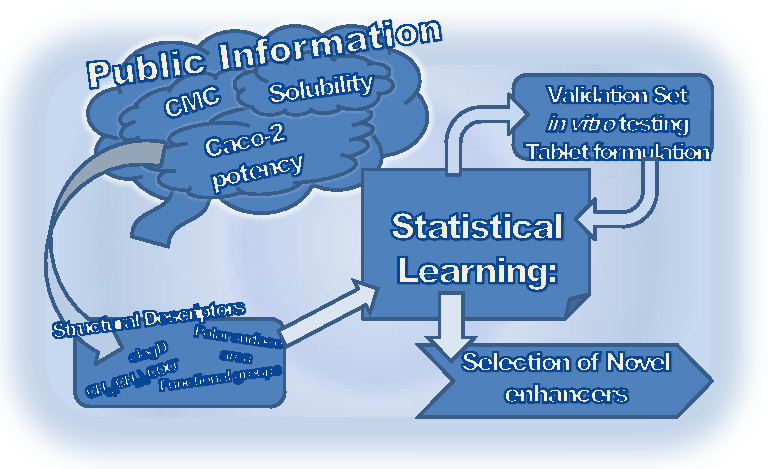
\includegraphics{graphics/workSummary_130mm.pdf}
\caption{Project idea. This figure was first designed for PhD-related presentations given by the author.}
\end{figure}


\begin{figure}[ht]
\label{devel_fassif}
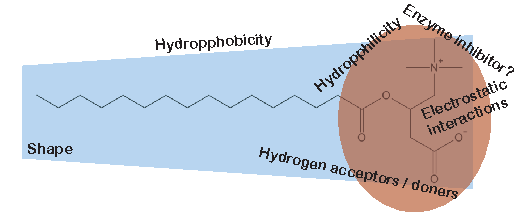
\includegraphics{graphics/typeOfSurfactant.pdf}
\caption{how does a surfactant like enhancer look like. This figure was first designed for PhD-related presentations given by the author.}
\end{figure}

\begin{figure}[ht]
\label{devel_fassif}
\includegraphics[width=\textwidth, height=\textheight, keepaspectratio]{graphics/predictPotencySummary.pdf}
\caption{Outline how to predictions are made. This figure was first designed for PhD-related presentations given by the author.}
\end{figure}

The decision tree ensemble random forest have a series of useful diagnostics which have been used in this thesis work.

\newpage

\includepdf[pages={1-},scale=0.90,pagecommand={\pagestyle{myruled}}]{chapters/predictPotencyArt.pdf}
